Before we can discuss how the Pellerhaus will be reconstructed by the projection of point clouds as 3D panoramas, it is necessary to build up some fundamental knowledge about the history of the Pellerhaus, and define what a 3D panorama is and what properties it has. Those fundamentals will enable us to start with the creation of software tools or 3D models that build upon this basic information. First, we establish a brief historic review of the art epoch in which the Pellerhaus was built to understand the underlying principles of the way it was designed and what it communicated by its authentic style. Secondly, this report presents a definition of the term "3D panorama" and explains how such a panorama is created from a high-level perspective which prepares the reader for the low-level details in the next chapter.

\section{Historical fundamentals}

\subsection{Renaissance}

We can group certain historical time periods by name. For example, the time period between the years 400 to 1499 (often referred to as the 5th and 15th century, respectively) are called the Middle Ages. The time period after the year 1500 (or in other words after the 16th century) is known as Modern History. We want to take a closer look inbetween those two time spans, namely the period from the 14th to the 17th century. This is where the Renaissance art epoch was active and the Pellerhaus Nürnberg was built. Renaissance literally means "rebirth" when translated from French. In the Late Medieval period the Renaissance started as a cultural movement in Italy first, and subsequently spread across the rest of Europe. Because it is located between the aforementioned time epochs it is considered to be the bridge between them. The start of the Renaissance in Italy was fostered by the support for artistic movements from powerful and dominant families like the Medici, comparable to today's art patronage of digital artists by larger companies (see Voss 2014 \parencite{art_patronage_google} in The Guardian). The Medici family in Florence poineered the banking system and therefore introduced a commercial revolution to finance the Renaissance.

The Fall of the Constantinople in 1453 at the hands of the Ottoman Turks caused Greek scholars to migrate towards the west. When they arrived in Italy they spread their wisdom and knowledge of ancient Greece and Rome through all the major city states across the Italian peninsula, such as Florence, Venice, Milan, and Rome, during the Renaissance papacy. Thus, the influence of the Renaissance affected the questioning of many aspects in life, like literature, philosophy, art, music, politics, science and religion. Scholars established new methods of study and introduced realism and human emotion in art. 

The principles expressed by the Renaissance are a cultural revival of the ones developed in the ancient Greek and Roman Empires, where for instance in architecture the most representative building was said to be a temple (see Wikipedia 2015 \parencite{wiki:Ancient_greek_roman_principles}, Architecture section). Since these principles were not applied uniformly all over Europe, widespread educational reform was gradual, though it had a major impact in all aspects of life. In politics it was the base of the conventions of diplomacy, and in science the renaissance brought an increased reliance on observing nature instead of pure superstition. The greatest impact, however, was on arts, with discoveries made by famous artists like Leonardo da Vinci and Michelangelo. To summarize, the Renaissance could be considered as an attempt to study and improve the physical world by reviving ancient ideas and principles on the one hand and new approaches to thoughts on the other hand.\\

This revival based on ancient Greek and Roman culture is observed in Renaissance Architecture as well. It followed Gothic architecture and was succeeded by Baroque architecture. The typical Renaissance style in architecture is described by Wikipedia \parencite{wiki:Renaissance} as follows:

\blockquote{
	Renaissance style places emphasis on symmetry, proportion, geometry and the regularity of parts as they are demonstrated in the architecture of classical antiquity and in particular ancient Roman architecture, of which many examples remained. Orderly arrangements of columns, pilasters and lintels, as well as the use of semicircular arches, hemispherical domes, niches and aedicules replaced the more complex proportional systems and irregular profiles of medieval buildings.	
}

\textbf{Renaissance Architecture in Germany}\\

The arrival of Renaissance architecture in Germany was inspired by German philosophers and artists such as Albrecht Dürer and Johannes Reuchlin. They travelled to Italy, where they learned more about its advanced artistic world. Although the religious turmoil caused by the Protestant Reformation was frequently depicted in art or literature, gothic and medieval scholastic philosophy remained dominant until the end of the 15th century. When Emperor Maximilian I of Habsburg (1493-1519) rose to power, the Renaissance became popular in Germany, too. Maximilian I was the first true Renaissance monarch of the Holy Roman Empire.

There are several examples of early Renaissance architecture in Germany, such as the Landshut Residence or the Augsburg Town Hall, both located in the Free State of Bavaria in the south of Germany. Furthermore the largest Renaissance church was also built in Bavaria. Sir Wiliam V, Duke of Bavaria, had to raze 87 houses, ignoring the protests of the citizens, to construct the St. Michael's Church in Munich between 1583 and 1597.

Along the Weser river in central Germany a specific regional variant of architectural style called the "Weser Renaissance" has been preserved in unusually high density in towns and cities of that region. This was caused by the slow economic recovery of the region from the effects of the Thirty Years War (1618 - 1648 ) which made them unable to transform their architecture to baroque style (see Wikipedia 2015 \parencite{wiki:GermanRenaissance}).

Nuremberg had substantial achievements in the field of architecture around 1600 as well. Some of the most popular projects are described by Mährle (2000) in his book "Academia Norica" \parencite{bookAcademiaNorica} which is translated by the author from German as follows: 

\blockquote{
	Significant public and private buildings have been built between the end of the Second Margrave War and the beginning of the Thirty Years' War.
	
	The first big construction project after the end of the war against Albrecht Alcibiades was the fortification of the defense structures. During 1556-1564, the wall ring was improved and the towers of the five main gates (Laufer Tor, Spittlertor, Frauentor, Neutor, Vestnertor) were surrounded by a stone wall. This was inspired by the towers of Castle Sforza in Milan, Italy.
	
	Additional important public buildings were realized by the city builder Jacob Wolff der Ältere (1596-1612) and his son Jacob Wolff der Jüngere (1612-1620) during that time. The most important ones have been the construction of the Fleischbrücke inspired by the Ponte Rialto in Venice (after 1596), the Wöhrder Torbastei (1613/1614), the master builders' house on the Peunt (1615) and especially the city hall, which was inspired by late renaissance style palaces in Italy (1616-1622).
	
	Besides the public buildings there were several considerable private structures created around 1600. They mostly haven't been commissioned by patricians but rich merchants. The most important ones have been the Toplerhaus (1590), the Fembohaus (1591) and the Pellerhaus (1602-1607).
	
	At the same time many manors in the land domain of Nuremberg have been rebuilt in the following decades after the Second Margrave War.	
}


\pagebreak

\subsection{Pellerhaus}

The Pellerhaus was built between 1602 and 1605 and considered one of the most magnificient examples of a town house in German Renaissance architecture.

\begin{wrapfigure}{r}{0.5\textwidth}
	
	\centering
	
	\includegraphics[width=0.48\textwidth]{Pellerhaus_1905_AF.jpg}
	\hbox{\scriptsize Credit: Altstadtfreunde Nürnberg e.V.}
	\caption{Pellerhaus around 1905}
	\label{fig:pellerhaus_1905}
	\vspace{-10pt}
	
\end{wrapfigure}

The house was commissioned to be constructed by the wealthy trading company Viatis-Peller, which was in the posession of the greatest assets at that time. Bartholomäus Viatis gave the Pellerhaus to his son-in-law Martin Peller where it remained in the posession of the Peller family until 1828.

The house changed owners several times during the subsequent 100 years until it was purchased by the mayor of Nuremberg Hermann Luppe in 1929. Acquring the house assured a proper maintenance of this historic landmark by the city. It was estimated that a full reconstruction would need the budget of a Martin Peller to succeed. Nuremberg felt responsible for maintaining the beauty of the Pellerhaus at that time and financed a restoration of critical parts of the building. Hence, it started a refurbishment program between 1931 and 1934 for the Pellerhaus, where the focus was put on restoring the delightfulness of the court yard and the rear facade. The red facades have been cleared up and new stone details have been redone by hand. Artists were careful to keep all of the small details and not to recreate the house in a more modern style. The Pellerhaus was saved. Luckily it was at that time that a vast documentation of the historic Pellerhaus was created. This 1930's restoration is incredible worthy today. Hundreds of plans and photos document every detail of its facade. Without that documentation a reconstruction would have been extremely difficult today (see Pellerhaus Magazin 2013 \parencite{afPellerhausMagazin02}).

Unfortunately, Nuremberg suffered from an Allied aerial bombing on January 2nd, 1945, as a result of World War II. It was the most severe attack made by aerial bombardment at that time. Nearly 1,800 people were killed that day. This Area Bombing Directive was issued by the British Air Ministry which directed the Royal Air Force to concentrate their attacks on factories and industry buildings in general. The objective of the directive was to focus the attacks on the enemy morale. Hence, the bombardment is often called „Morale Bombing“. Many buildings were transformed into a leveled surface after the removal of the debris remaining from the attack. The bombed areas today present either completely new buildings or reconstructed ones. The Pellerhaus is a building that has been reconstructed after World War II.

\pagebreak

\begin{wrapfigure}{l}{0.5\textwidth}
	
	\centering
	
	\includegraphics[width=0.48\textwidth]{Pellerhaus_2015_AK.jpg}
	\caption{Pellerhaus 2015}
	\label{fig:pellerhaus_2015}
	\vspace{-10pt}
	
\end{wrapfigure}

The reconstruction was initiated in 1955. It only preserved the base floor in its historic state, due to the fact that major parts of it survived the bombing. From the first floor upwards, the facade of the Pellerhaus changed dramatically and only served a pure functional purpose, as room was needed to accomodate the new City Library and Archive. It was almost decided to completely embed the Pellerhaus into the Library which had been built to the right of it, but a movement within the city prevented that. An old arch was completely destroyed to connect the Pellerhaus with the Library, which was criticized as being senseless. Only some column bases and capitals remained in the inner courtyard, ready to be build into the southern part of the court. So all six arcs, the small passage next to the front-facing house and the adjacent facade part of the northern court facade needed to be recreated. In the end, the old style Pellerhaus was combined with a new style to allow at least some experience of the old state. The reconstruction of the base floor was finished in 1957. The upper floors - and therefore all reconstruction efforts - were finished by 1960. At that time people realized that a full reconstruction might happen some day, although the individual storey heights differ from the original. Conversely, when a secondary school was built on top of the back-facing house in 1972/73, almost any hope of a full reconstruction of the Pellerhaus was dashed (see Pellerhaus Magazin 2012 \parencite{afPellerhausMagazin01}). \\


\begin{figure}[h]
	\centering
	\begin{subfigure}[b]{0.3\textwidth}
		\centering
		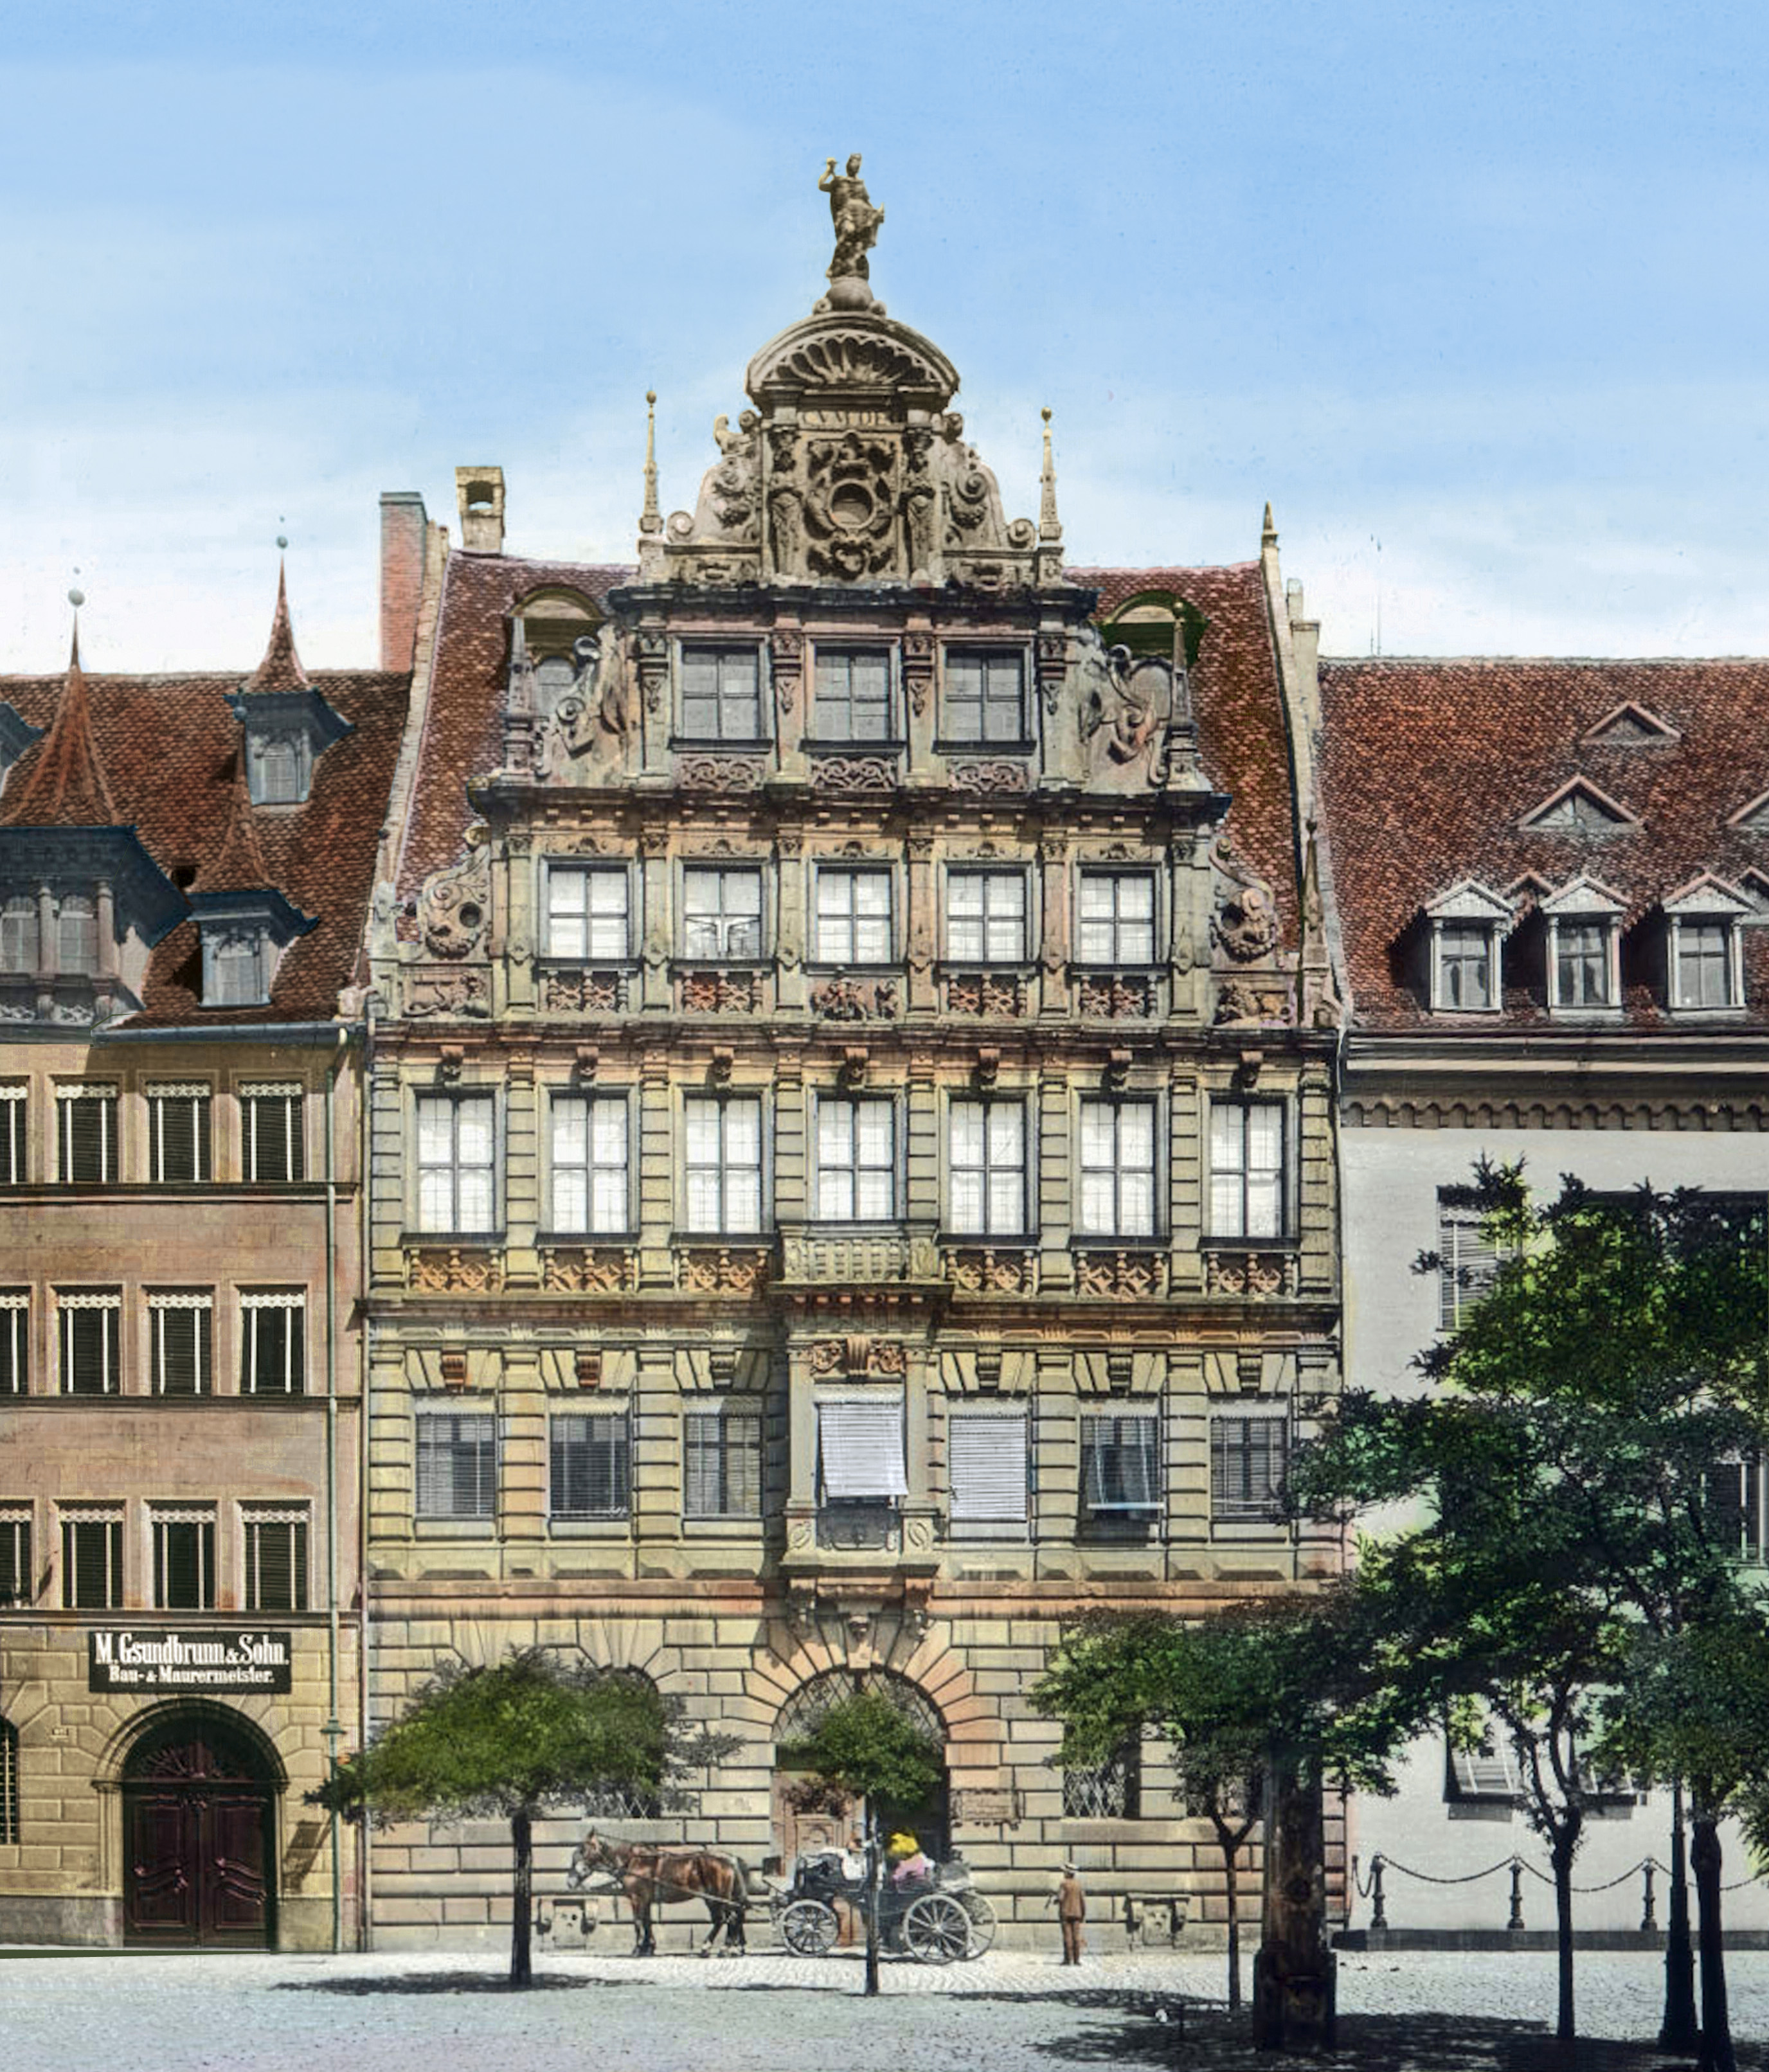
\includegraphics[width=\textwidth]{Pellerhaus_before1945_Carl_Simon_United_Archives.jpg}
		\hbox{\scriptsize Credit: Carl Simon United Archives}
		\caption{before 1945}
		\label{fig:pellerhaus_historic}
	\end{subfigure}
	\hfill
	\begin{subfigure}[b]{0.3\textwidth}
		\centering
		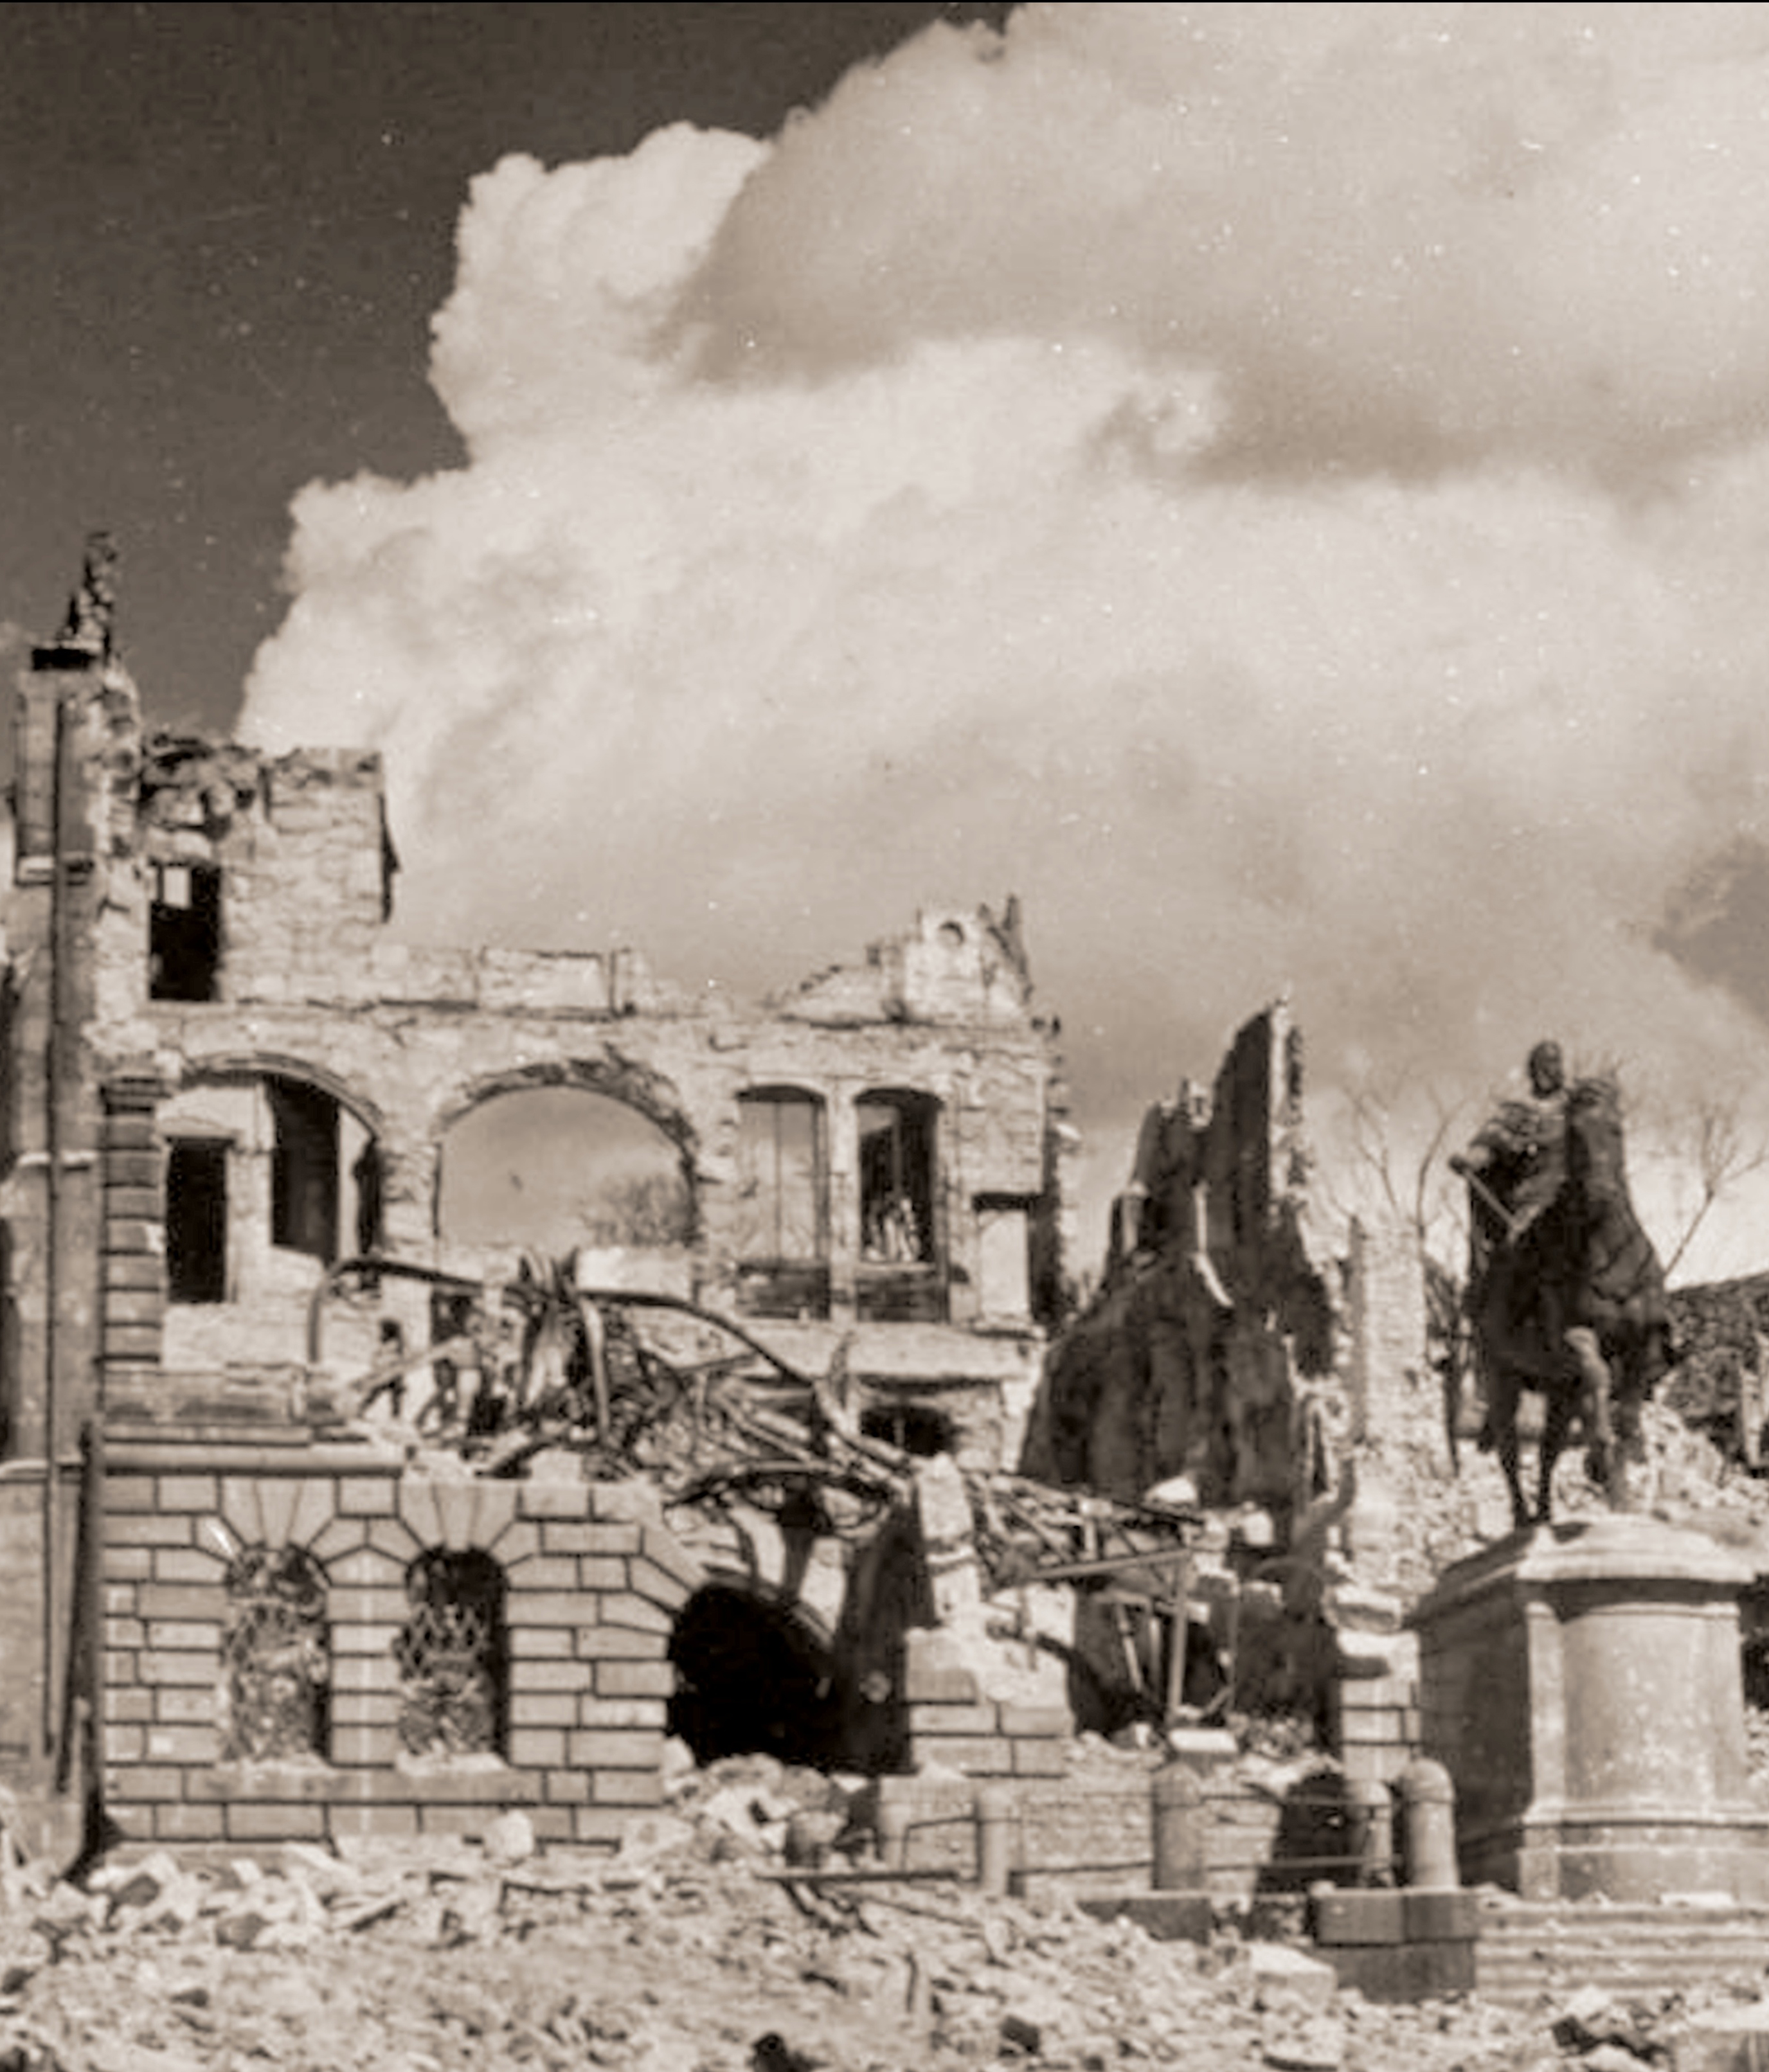
\includegraphics[width=\textwidth]{Pellerhaus_1945_Life_Archive.jpg}
		\hbox{\scriptsize Credit: Life Archive}
		\caption{Pellerhaus 1945}
		\label{fig:pellerhaus_destructed}
	\end{subfigure}
	\hfill
	\begin{subfigure}[b]{0.3\textwidth}
		\centering
		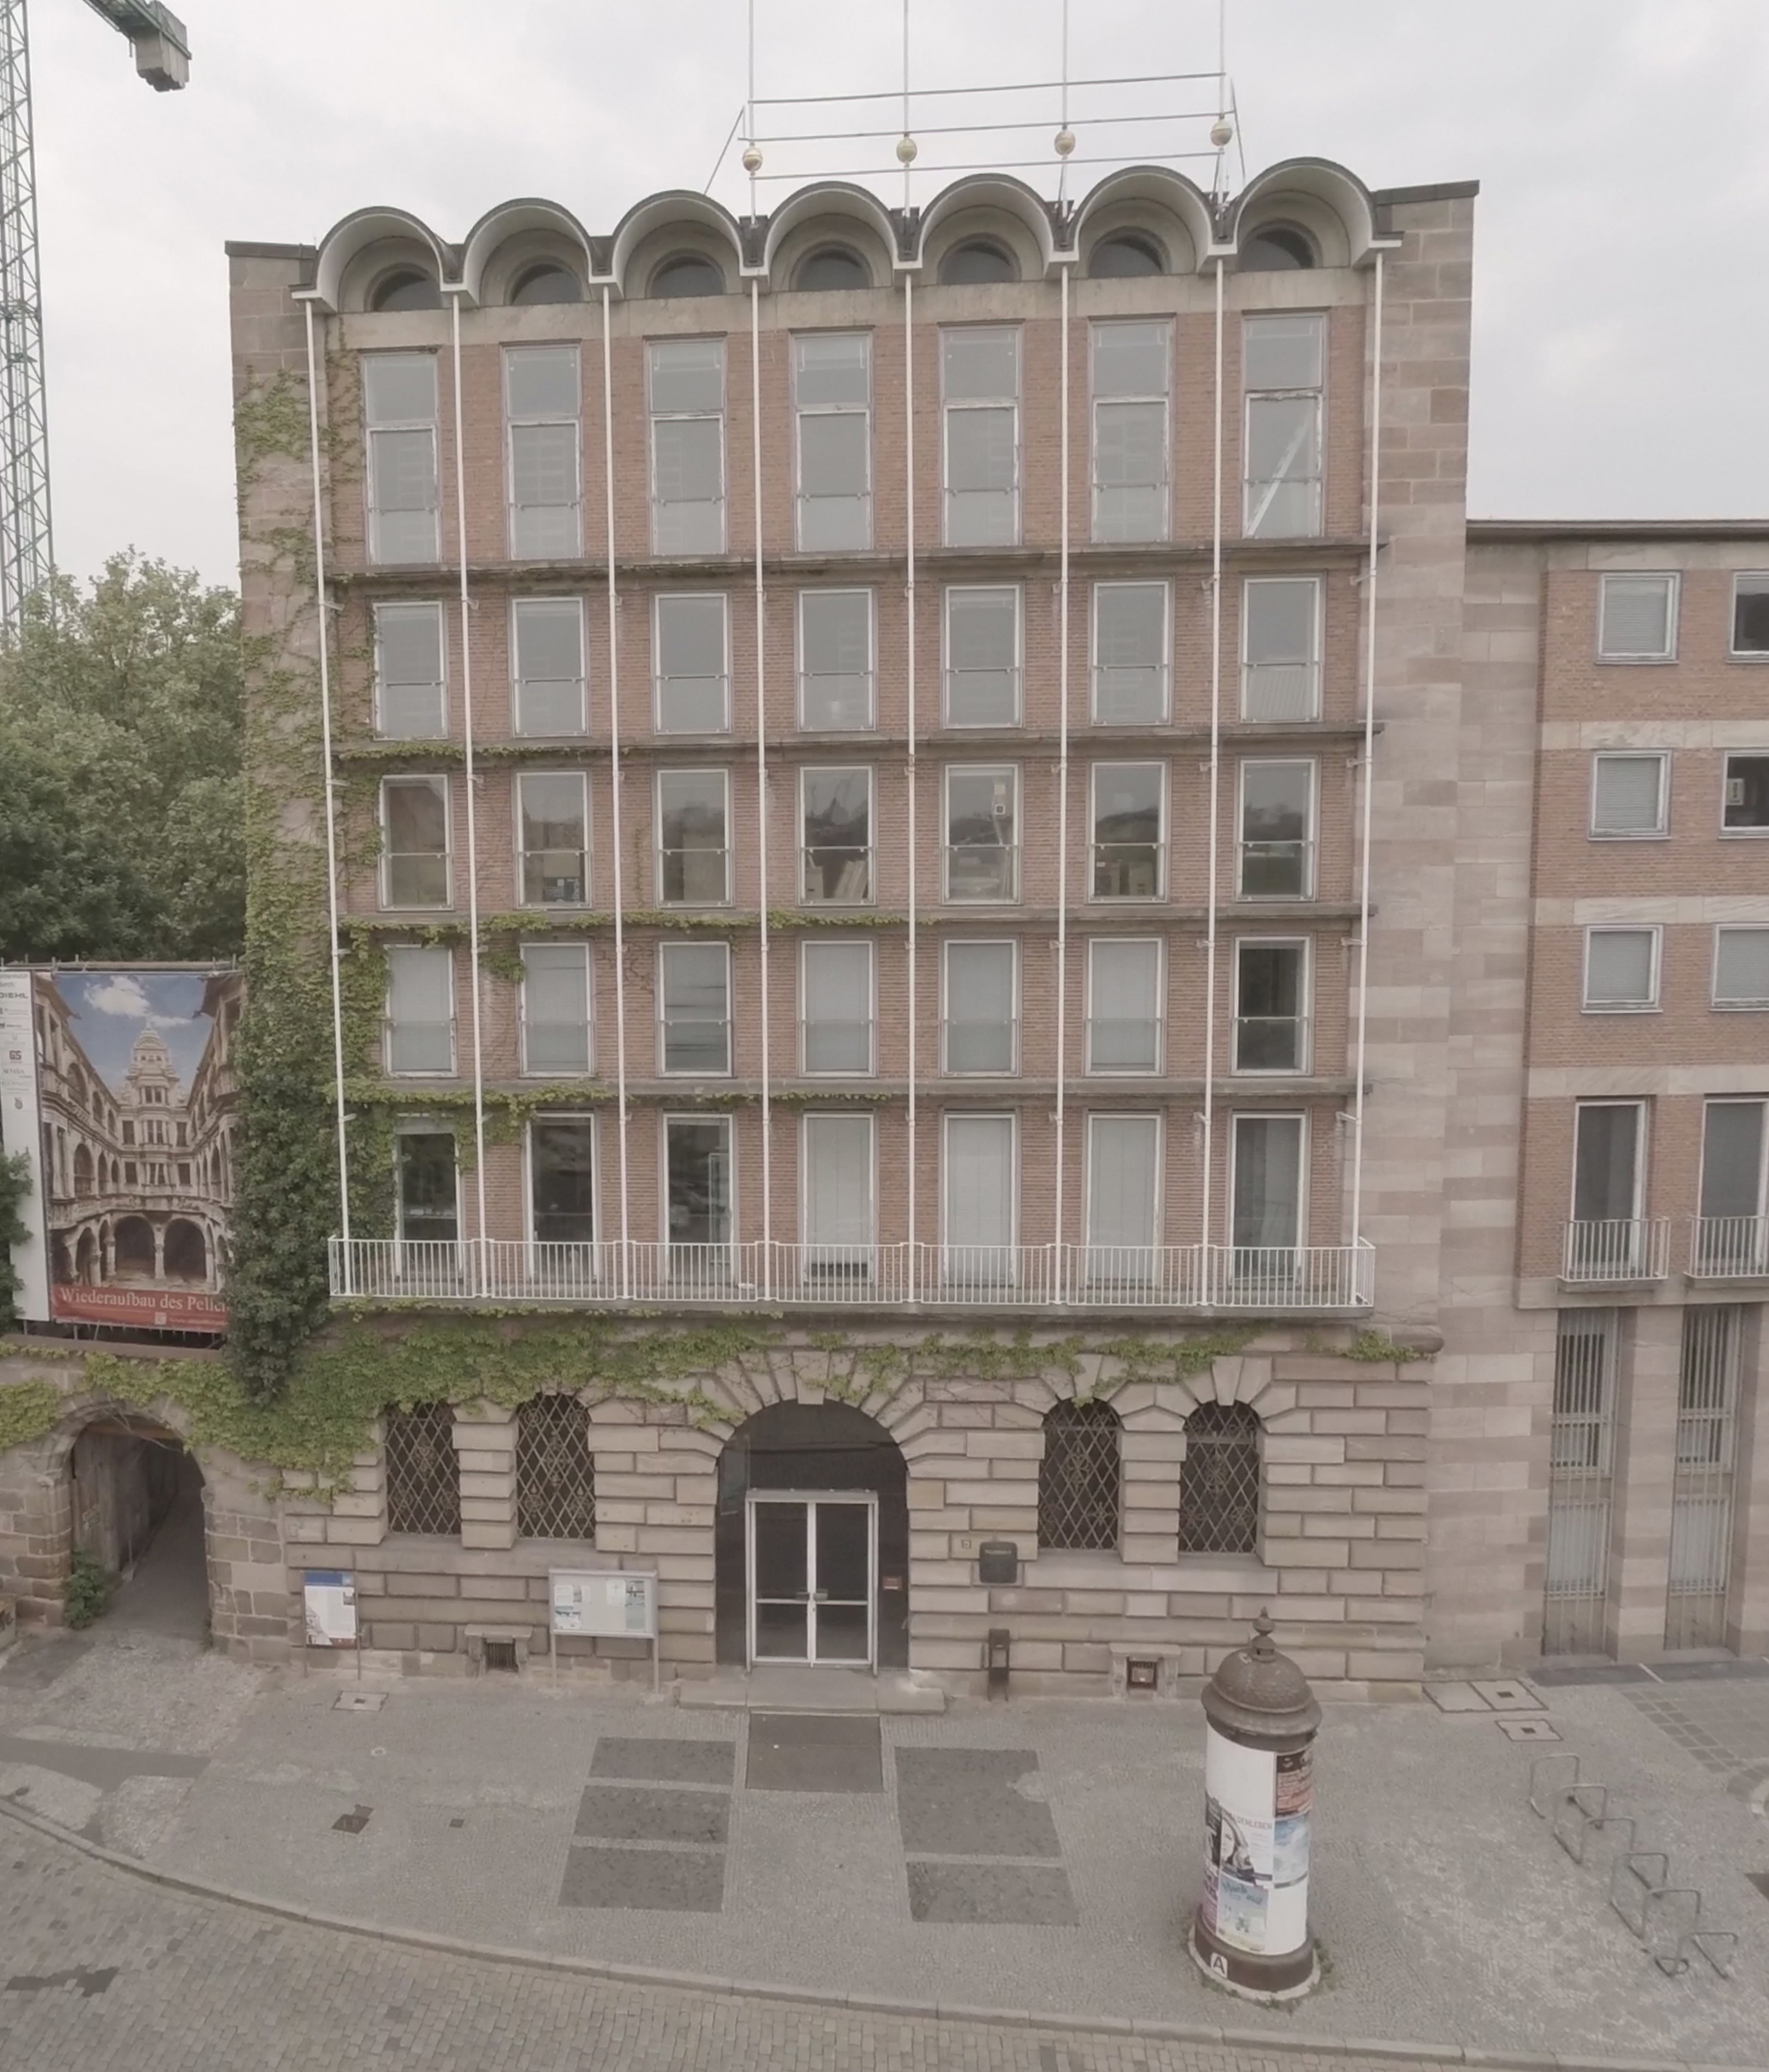
\includegraphics[width=\textwidth]{Pellerhaus_after1945_AK.jpg}
		\hbox{\scriptsize }
		\caption{after 1945}
		\label{fig:pellerhaus_modern}
	\end{subfigure}
	\caption{The Evolution of the Pellerhaus}
	\label{fig:pellerhaus_states}
\end{figure}

In 2005 a new initiative was launched, which had the goal of reconstructing the Pellerhof, which is the inner courtyard of the Pellerhaus. With its groined vaults, it is an artistic piece of architecture. The association Altstadtfreunde e.V. created a flyer \parencite{afWiederaufbauDesPellerhofes} which includes a wonderful description of the Pellerhaus that has been translated by the author from German:

\blockquote{
	Before destruction, the Pellerhaus was one of the main sights of Nuremberg. The architecture seems to be the most honorable performance of the local art of construction. Its inner court was considered the probably most beautiful arcade court.\\
	As the city descended into shatters in 1945, there were only a few remains of the Pellerhaus. The front-facing house was rebuilt in a modern form 1957 on top of the reconstructed hall. An enourmous effort was done by complementing the courtyard, it was discontinued 1959, though.\\
	Not until 2005, 60 years after the destruction, the Altstadtfreunde took the initiative to continue the former abandoned construction of side wing and rear house facade.\\
	With the accurate documentation of the pre-war level it is possible to do those court additions with extraordinary accuracy. October 2008 layed the foundation block of building the courtyard completely via donations.\\
	Since then with the well corner, side wings and eastern backyard gallery crucial parts have been able to get restored from the old building.\\
	With your donation or by purchasing a symbolic block of stone you can help to make one of the greatest achievements of German Renaissance come alive in its historic state.\\
	At the time when the merchant Martin Peller started with building his house in 1602, he also layed the foundation block to what later entered as the most magnificient bourgeois house into the history of art. The notion of building an arcade court was not new in Nuremberg. There have been hundreds of gallery courts in the city. Many of them with tracery breastwork made of stone. Though, the Pellerish courtyard bested everything that has been known at that time:\\
	On the two long sides it was flanked by noble three-story arcades, with a clear and symmetric structure, though with a rich and filigreed ornamentation. While skimming along it, ultimately the show façade caught the eye with a glorious gable. Seldom one can find forms of the italian renaissance merged with local sensuous enjoyment in such a happy way. Antique style pillars accompany the individual floors, obelisks stretch up into the sky and still the appearance was entirely different than in Italy. The Pellerhof, as a Middle European counterpart to the wonderful arcade courts of Italy, is an indispensable part of european architecture.\\
}

This project is still active today and the Pellerhof has almost been fully reconstructed by the Altstadtfreunde Nürnberg e.V. at the time of this writing. The build process was mainly based on photos and the remains of the western side. Measurements have been extracted by examining the remains including profiles, design of capitals and ending stones. Overall forms were reconstruced with the help of historic photos. New constructions were needed for the differing tracery of balustrade areas. It was a stroke of luck that the historic documentation of the house is extensive. This helped reconcile differences of geometrically correct constructions with the new build. The Chörleins (a type of bay window) are also documented well enough to allow for a reconstruction. For example, there was an incorrect ornamentation of Chörleins at window lintels, sockets, and volutes when comparing the rebuild from 1950 with the original. The new build comes much closer to the Renaissance original. The Altstadtfreunde Nürnberg e.V. can proudly say that, with their restored state, the two time layers 1605/07 and 1957/59 form a harmonic unit. In April 2013 they moved newly produced stone blocks and a fully donated arc into the Pellerhaus. Once again, they noticed reckless deviation from consistancy. All of the six arcs have different spans and the alignment of the arcarde row is not straight, but has been – in its old parts – slightly bulged out. Though this might be due to the bombing destruction, the fact that the arc row doesn't continue horizontally but considerably descends from the front-facing house into the courtyard is notable.

Many of the facades of the buildings in Nuremberg have been painted red with white rectangles. The reason for this was that the look of mined stones varied considerably, so by painting them the houses had a united look. This color is also called the „Nürnberger Rot“ (Terra Norimbergensis rubra), because it looks like the local sand stone and the color powder comes from the rural area of Nuremberg. Unfortunately only a few color remains are left but it is enough to prove the colorfulness of the facade. After finishing the reconstruction in the courtyard, repainting the facades in the „Nürnberger Rot“ would be the right decision (see Pellerhaus Magazin 2014 \parencite{afPellerhausMagazin03}).

With the ongoing progress of the reconstruction of the Pellerhof, our research will examine ways to reconstruct the historic Pellerhaus facade as a 3D model.\\

\subsection{Architects of the Pellerhaus Nürnberg}

The Pellerhaus was constructed by the German architect Jakob Wolff der Ältere who was born in Bamberg in 1546. He accomplished several famous building projects in Nuremberg, such as the Fleischbrücke. He had two sons, Hans and Jakob Wolff der Jüngere. They were educated by their father and built the city hall of Nuremberg.

A detailed biography about the architects can be found in the Appendix (\ref{appendix_pellerhaus_architects}).

\section{3D Panorama}

The term "panorama" is defined by Wikipedia \parencite{wiki:Panorama} as follows:

%πᾶν and ὅραμα

\blockquote{
	A panorama (formed from Greek {$\pi\tilde{\alpha}\nu $} "all" + {$\ddot{o}\rho\alpha\mu\alpha$} "sight"), is any wide-angle view or representation of a physical space, whether in painting, drawing, photography, film, seismic images or a three-dimensional model. The word was originally coined in the 18th century[1] by the Irish painter Robert Barker to describe his panoramic paintings of Edinburgh and London. The motion-picture term panning is derived from panorama.
}

In simple words this means that we can create a two-dimensional image containing every view one can see from a fixed position. Below is an example how this could look for the Pellerhaus (see Figure \ref{fig:2d_panorama}):

\pagebreak

\begin{figure}[h]
	\centering
	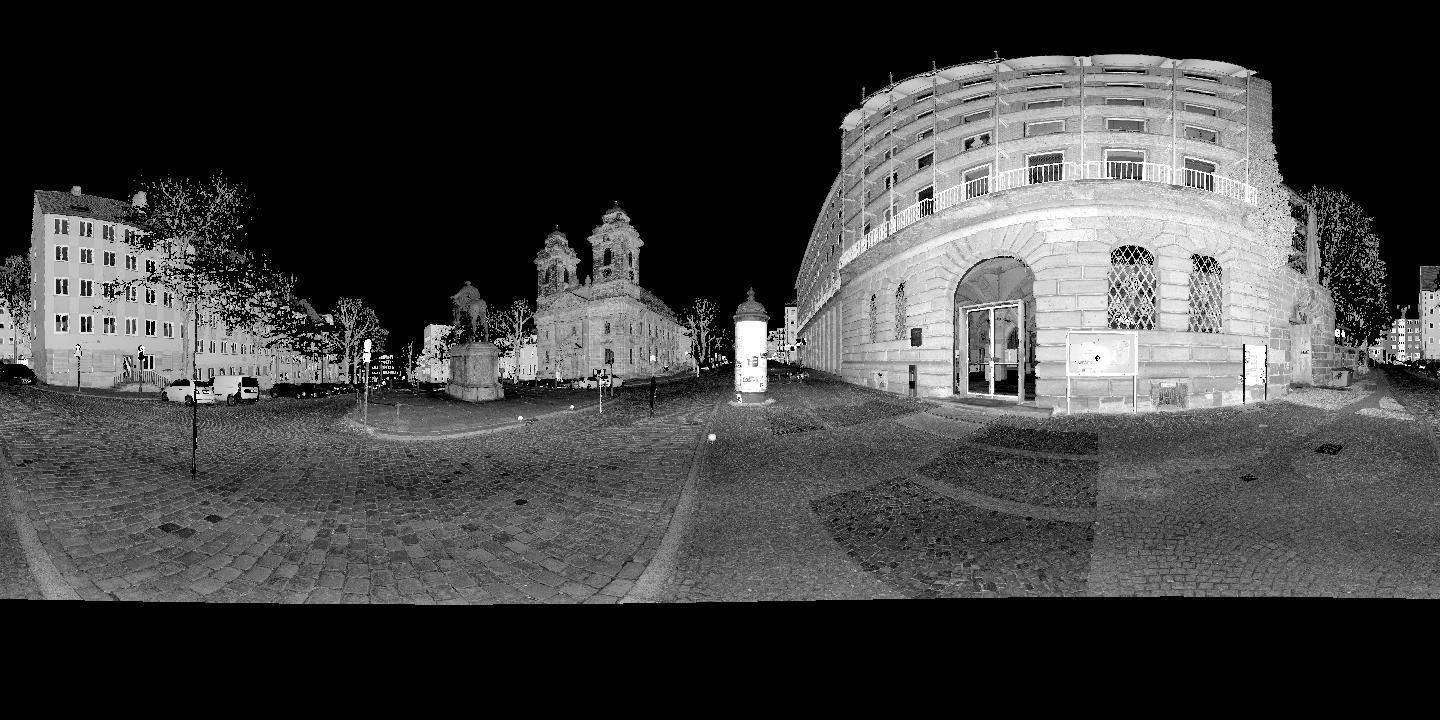
\includegraphics[scale=0.4]{2d_panorama_grey.jpg}
	\caption{2D Panorama of the Pellerhaus}
	\label{fig:2d_panorama}
\end{figure}

The image above was generated with the custom PointCloud2Blender (PC2B) converter software which will be discussed in detail in the next chapter. A two-dimensional panorama image depicts a full horizontal and vertical view of the location where it was taken. Please note that the example above is not a full vertical view, the reason being that this image was generated from a point cloud created by a laser scanner. Due to the tripod on which the scanner was mounted, the lower part of the scan is useless and therefore has been omitted by the scanning device. Additionally panorama images generated in PC2B are flipped horizontally (see Chapter \ref{section_optimizations}).

This two-dimensional panorama can now be converted to a three-dimensional panorama by simply mapping it onto a sphere, as shown here:


\begin{figure}[h]
	\centering
	\begin{subfigure}[b]{0.45\textwidth}
		\centering
		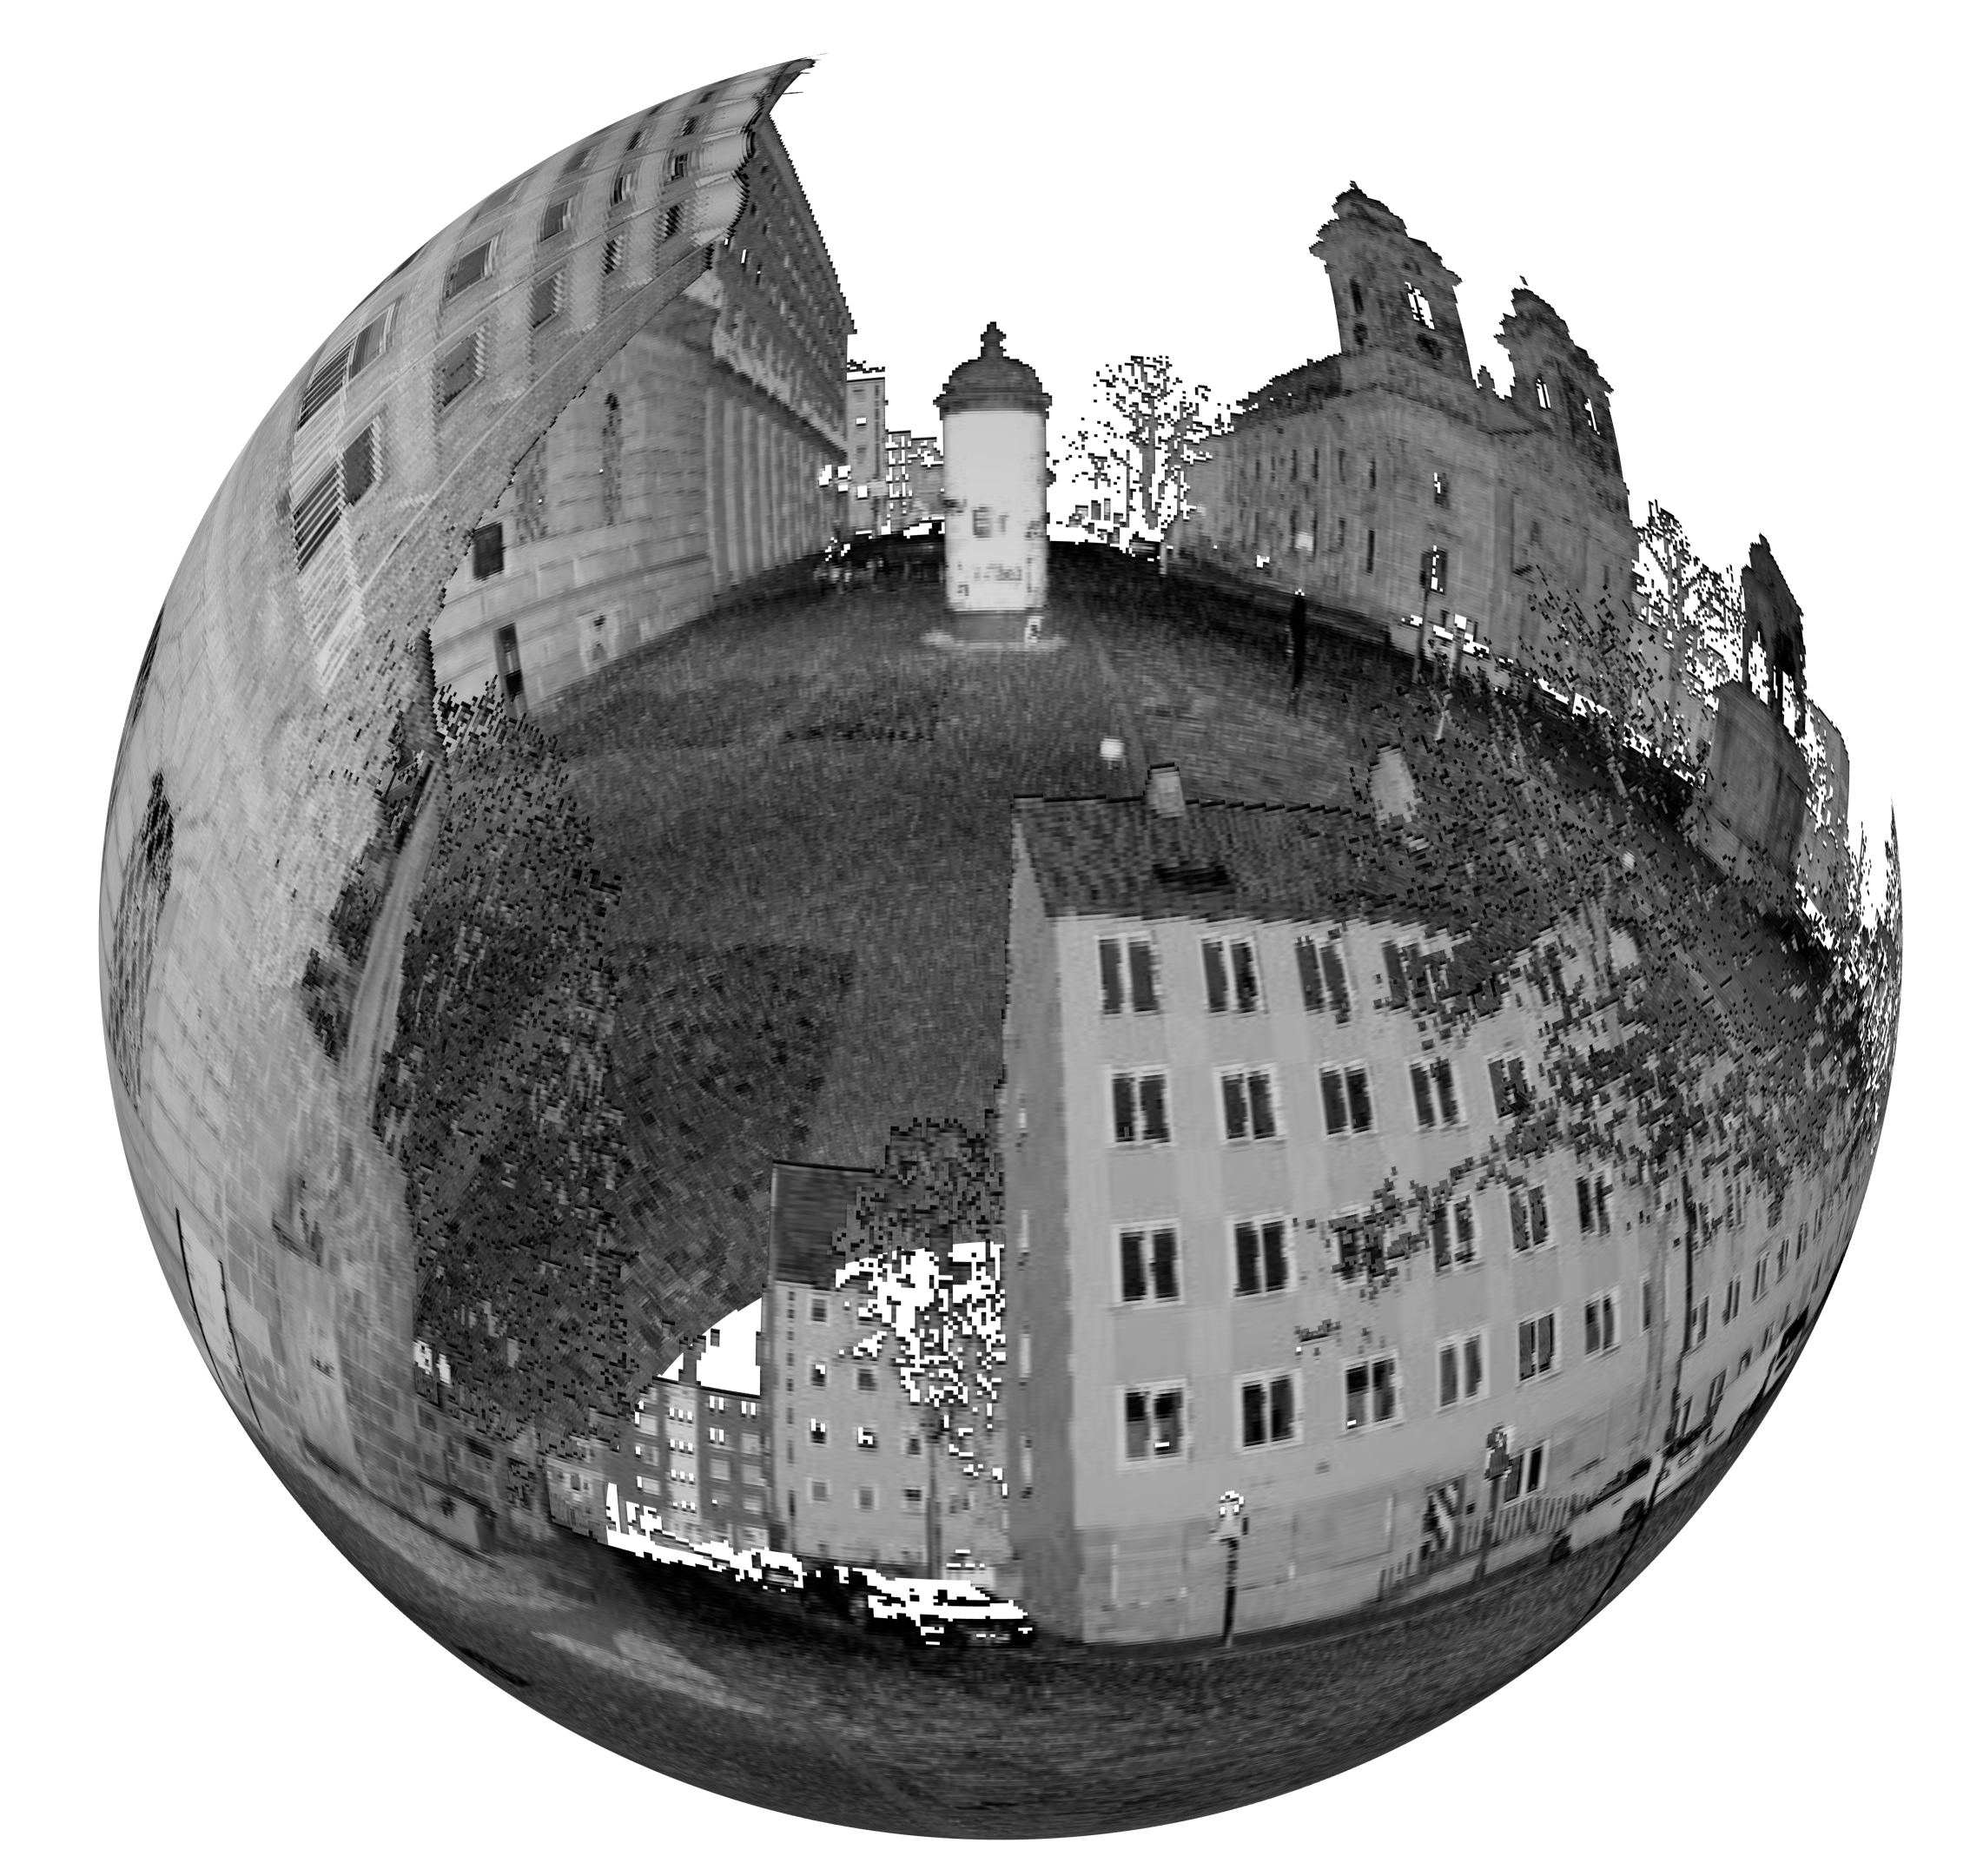
\includegraphics[scale=0.07]{3DPanorama_UnitSphere.png}
		\caption{2D Panorama mapped on a unit sphere}
		\label{fig:3d_panorama_unit_sphere}
	\end{subfigure}
	\hfill
	\begin{subfigure}[b]{0.45\textwidth}
		\centering
		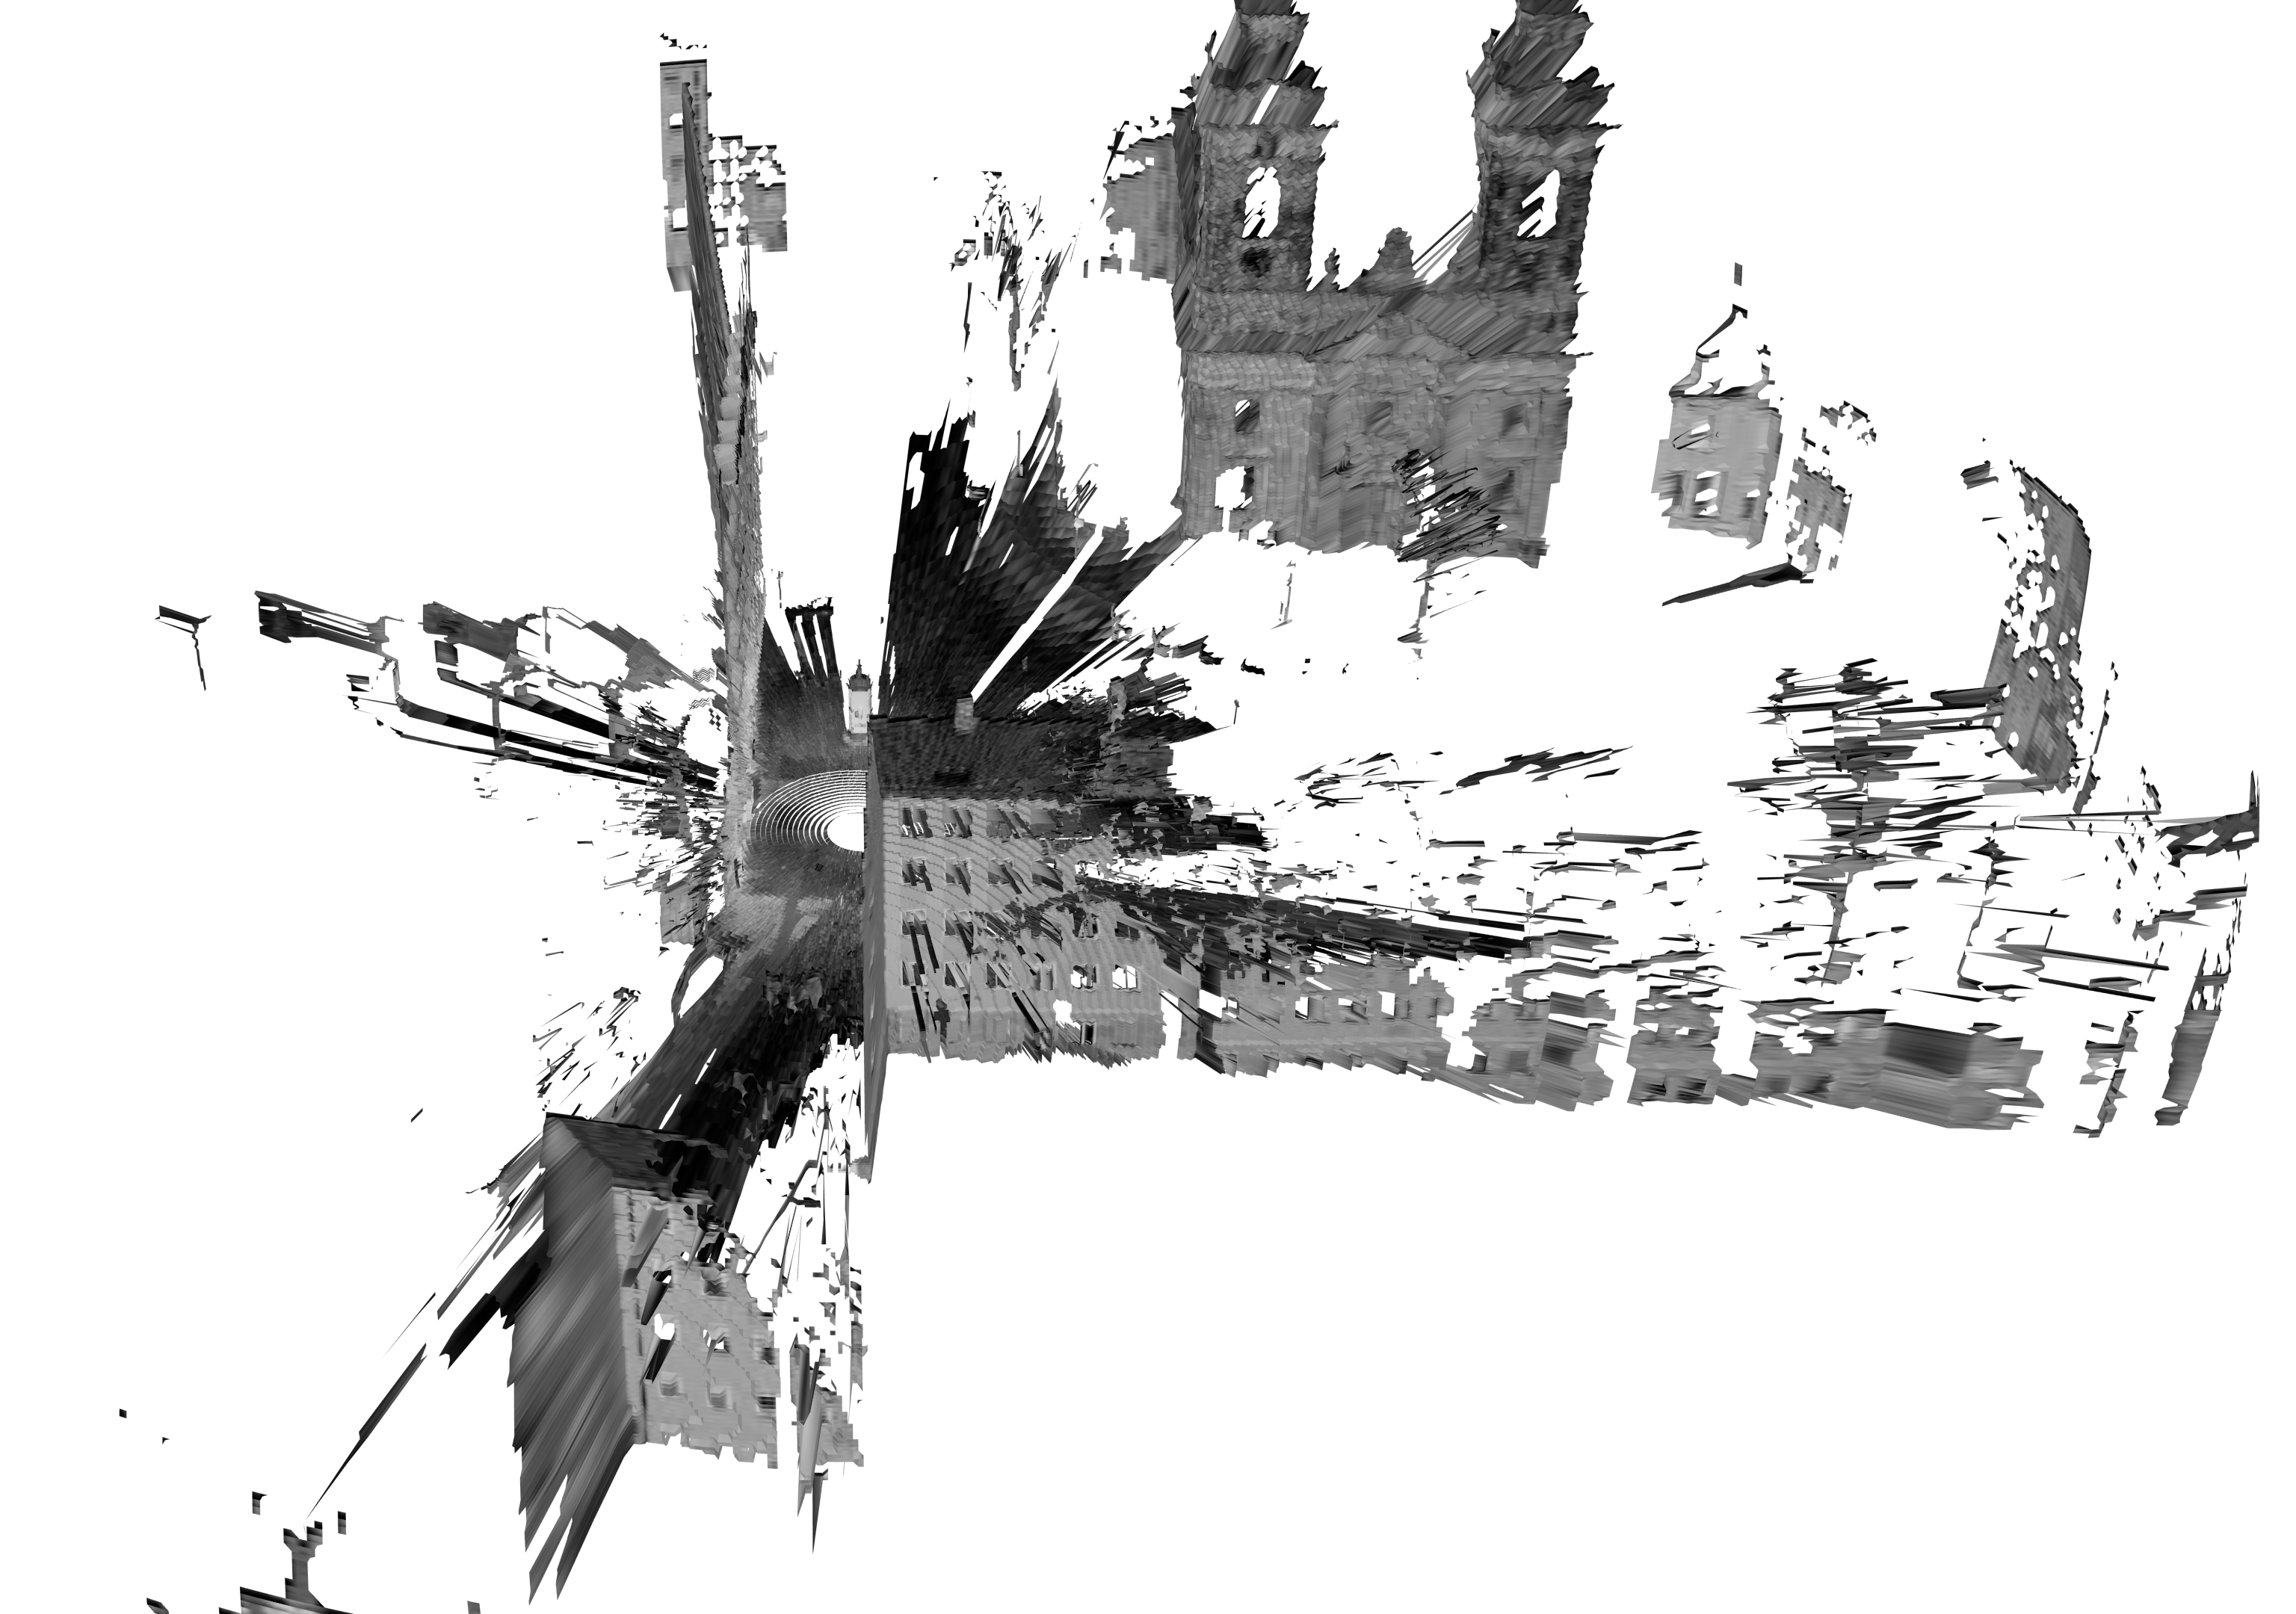
\includegraphics[scale=0.07]{3DPanorama_DepthSphere.png}
		\caption{The same panorama mapped on a sphere using individual distances}
		\label{fig:3d_panorama_depth_sphere}
	\end{subfigure}

	\caption{Mapping a two-dimensional panorama onto a three-dimensional sphere}
	\label{fig:3d_panorama}
\end{figure}

Placing a virtual camera in the center of the sphere makes it possible to visualize the complete three dimensional environment from one viewpoint.

3D Panoramas were given a great new use by the introduction of the Oculus Rift  (Oculus VR, \parencite{OculusVR}), and are increasingly used in film production as well. While this technique was used rather seldom in, for example, the Circle-Vision theaters in Walt Disney Theme Parks in 1955 (see Wikipedia 2015 \parencite{wiki:CircleVision}), today's hardware is becoming cheaper and faster to create such panoramas in real-time. The German FMX 2015, one of the biggest international conferences on animation, effects, games and transmedia, presented several software and hardware solutions that were able to stitch multiple video feeds into one panorama (see Kolor 2015 \parencite{kolorGoPro}). A very sophisticated example of using video panoramas combined with visual effects is Google ATAP ‘HELP’ (see CGMeetup 2015, \parencite{googleATAPHelp}), which is a video that can be viewed interactively on mobile devices from every angle by simply pointing the device in the desired direction.

\subsection{Creating panoramas} \label{section_creating_panoramas}

To create panoramic images it is necessary to map a three-dimensional environment onto a two-dimensional plane. This is accomplished by computing the spherical coordinates of every point in three-dimensional space. Without going into too much technical detail, we can either define a point in 3D space with its x, y and z coordinate (known as the cartesian coordinates) or with their horizontal angle displacement, vertical angle displacement and distance from the origin (which is known as spherical coordinates). The latter can be imagined as rotating and scaling a unit sphere until it intersects the point.

To clarify the process a little further, we provide a visual example. Consider the 3D point A at {$(1.0, 1.0, 1.41421)$}  in cartesian coordinates {$(x, y, z)$}. We need to align the x-axis of a unit sphere, labeled Point B, with point A (Figure \ref{fig:visual_coordinate_conversion_1}). To do so, we first rotate the sphere along its local z-axis by 45 degrees (Figure \ref{fig:visual_coordinate_conversion_2}). Secondly, we rotate it along its local y-axis by 45 degrees (Figure \ref{fig:visual_coordinate_conversion_3}). Finally we scale the unit sphere by 2 to align both points with each other (Figure \ref{fig:visual_coordinate_conversion_4}). Now we have calculated the spherical coordinates {$(\theta, \varphi, radius)$} which are expressed as {$(45.0^{\circ}, 45.0^{\circ}, 2.0)$} in degrees or as {$(\frac{\pi}{4}, \frac{\pi}{4}, 2.0)$} in radians. This process is visualized below:

\begin{figure}[h]
	\centering
	\begin{subfigure}[b]{0.24\textwidth}
		\centering
		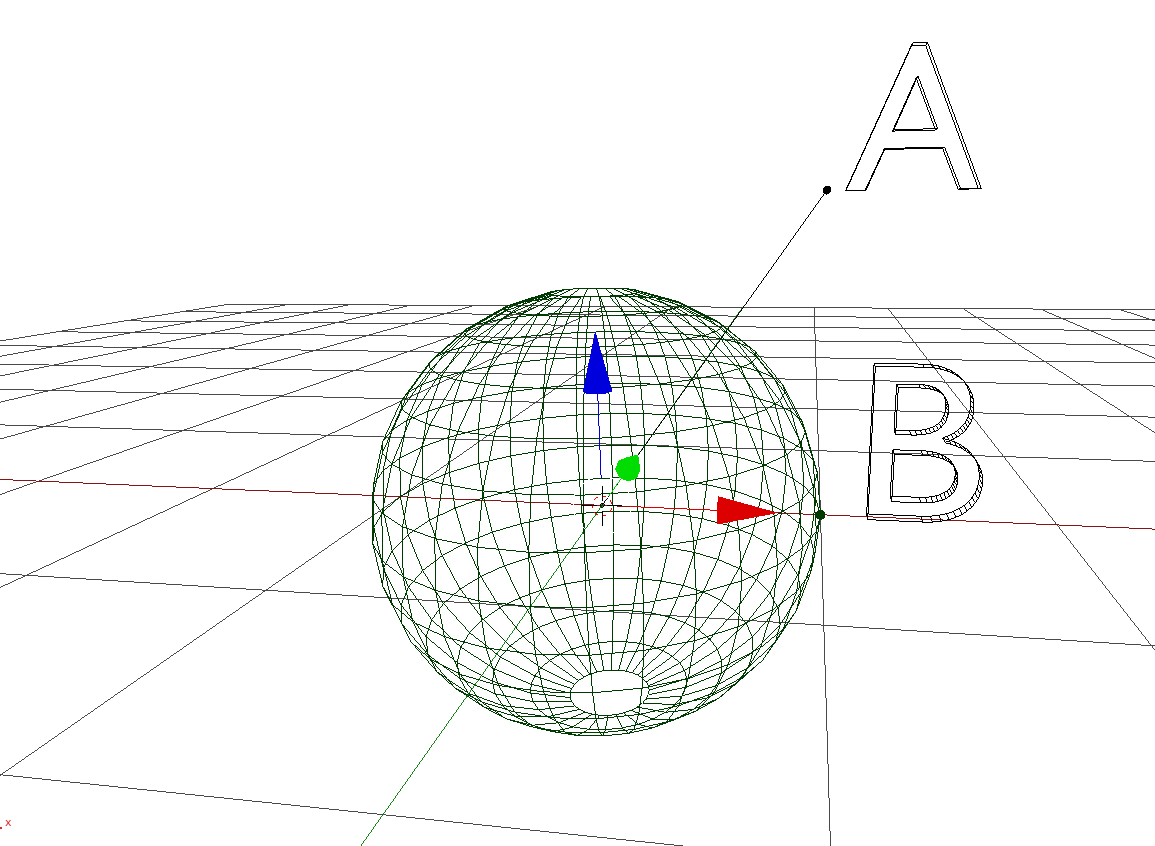
\includegraphics[scale=0.09]{Visual_Coordinate_Conversion_1.jpg}
		\caption{}
		\label{fig:visual_coordinate_conversion_1}
	\end{subfigure}
	\hfill
	\begin{subfigure}[b]{0.24\textwidth}
		\centering
		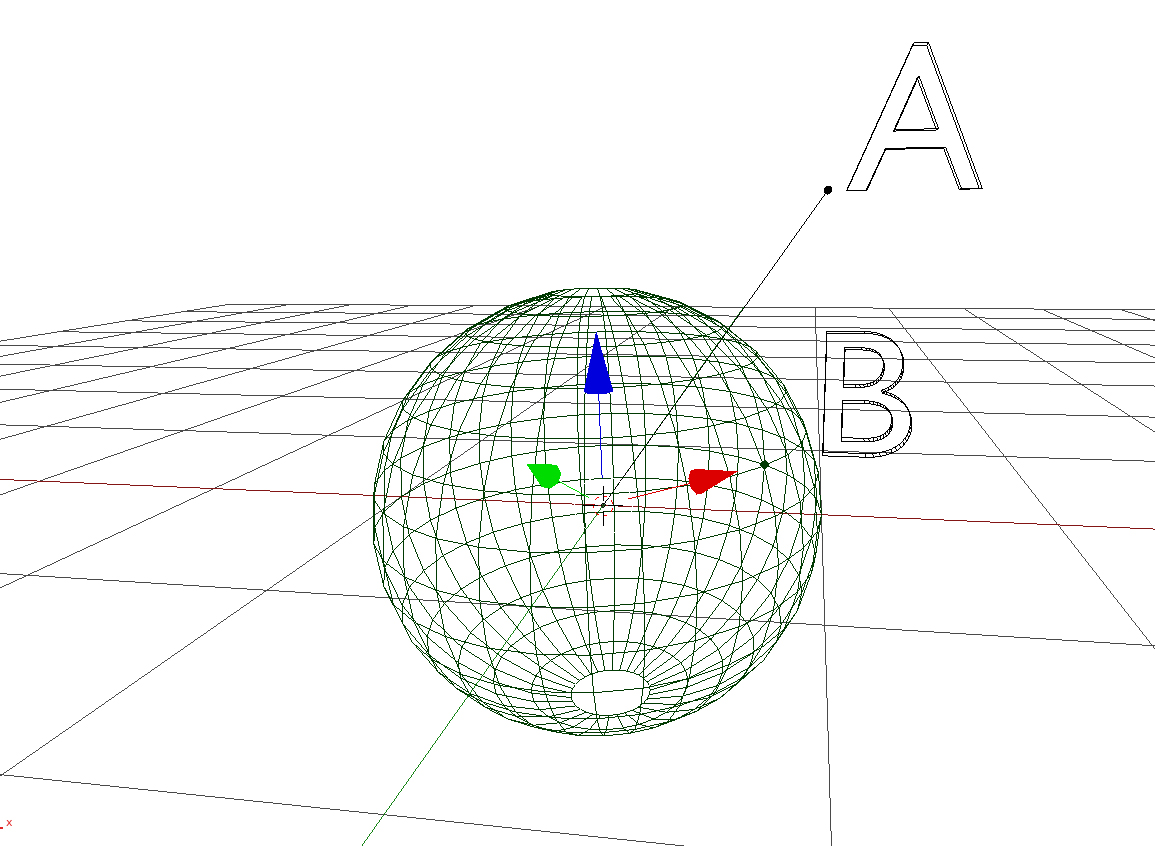
\includegraphics[scale=0.09]{Visual_Coordinate_Conversion_2.jpg}
		\caption{}
		\label{fig:visual_coordinate_conversion_2}
	\end{subfigure}
	\hfill
	\begin{subfigure}[b]{0.24\textwidth}
		\centering
		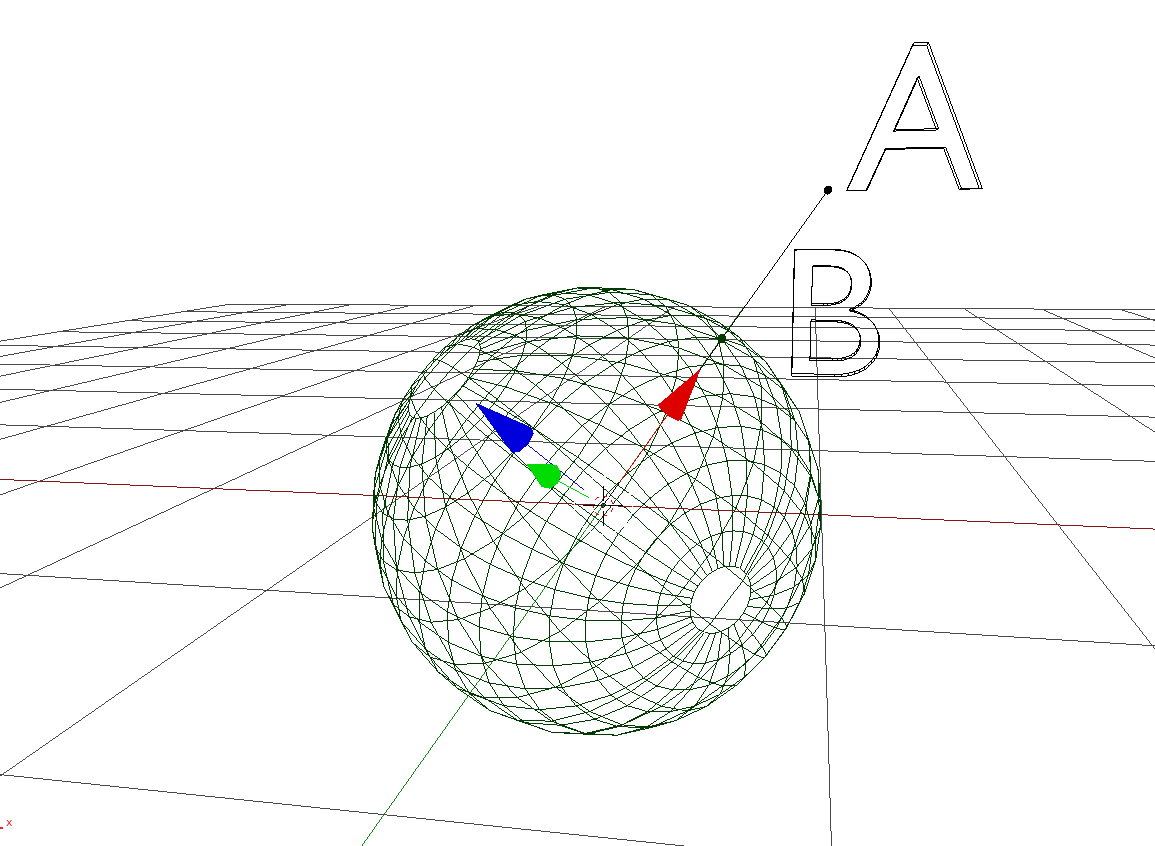
\includegraphics[scale=0.09]{Visual_Coordinate_Conversion_3.jpg}
		\caption{}
		\label{fig:visual_coordinate_conversion_3}
	\end{subfigure}
	\hfill
	\begin{subfigure}[b]{0.24\textwidth}
		\centering
		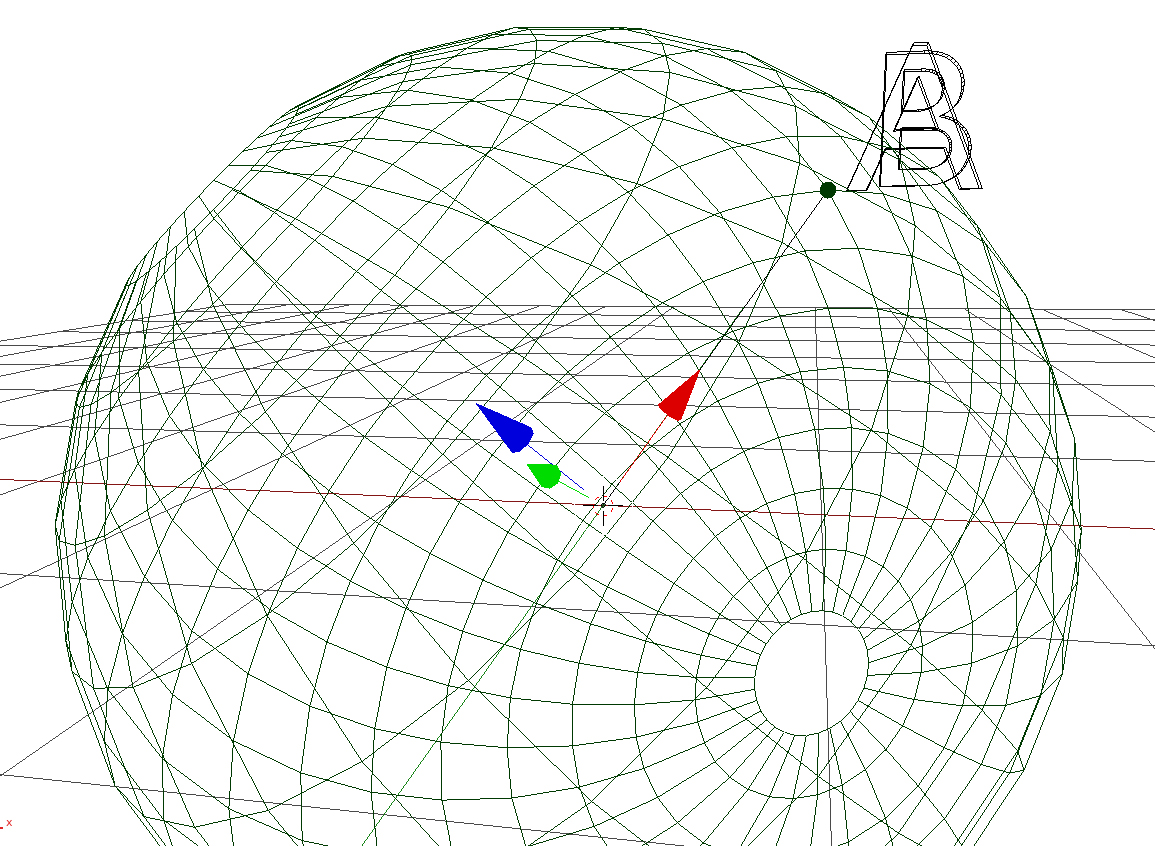
\includegraphics[scale=0.09]{Visual_Coordinate_Conversion_4.jpg}
		\caption{}
		\label{fig:visual_coordinate_conversion_4}
	\end{subfigure}
	
	\caption{Converting from cartesian to spherical coordinates, visually}
	\label{fig:converting_cartesian_to_spherical}
\end{figure}

The final image can be formed by mapping these spherical coordinates {$(\theta, \varphi, radius)$} to the image coordinates {$(x, y)$}. This is called panoramic projection.

There is a set of various types of projections used for panorama generation. A subset of them is introduced in the following section.

\subsection{Types of projections} \label{section_types_of_projections}

It is not possible to create a perfectly "flat" or two-dimensional representation of a sphere. There will always be distorted areas; thus it is necessary to choose the right projection type for every new task (see Furuti 2014 \parencite{panoramaProblem} ).

A study of implementing seven different projections was conducted by Houshiar et al. \parencite{houshiar2015a} in 2015. The findings of that study are the basis for our implementation in the converter software. We have implemented three projections, namely the equirectangular, cylindrical and mercator projections.

First, the equirectangular projection is the simplest type and can be implemented very quickly, as the spherical coordinates {$\theta$} and {$\varphi$} are mapped directly to the x and y coordinates of the two-dimensional image without any transformation.

Second, the cylindrical projection is similar, but the vertical mapping is transformed. This can be envisioned by placing a sphere inside a cylinder. If light is emitted from the center of the sphere it is projected onto the cylinder. The projection keeps vertical lines straight, but horizontal lines are still curved. Furthermore, objects are stretched vertically, which becomes more prominent the closer they are to the north and south poles of the sphere.

Lastly, the mercator projection is a mapping that preserves angles locally (conformal projection). The distortions are less pronounced than equirectangular or cylindrical projections.

\begin{figure}[h]
	\centering
	\begin{subfigure}[b]{0.3\textwidth}
		\centering
		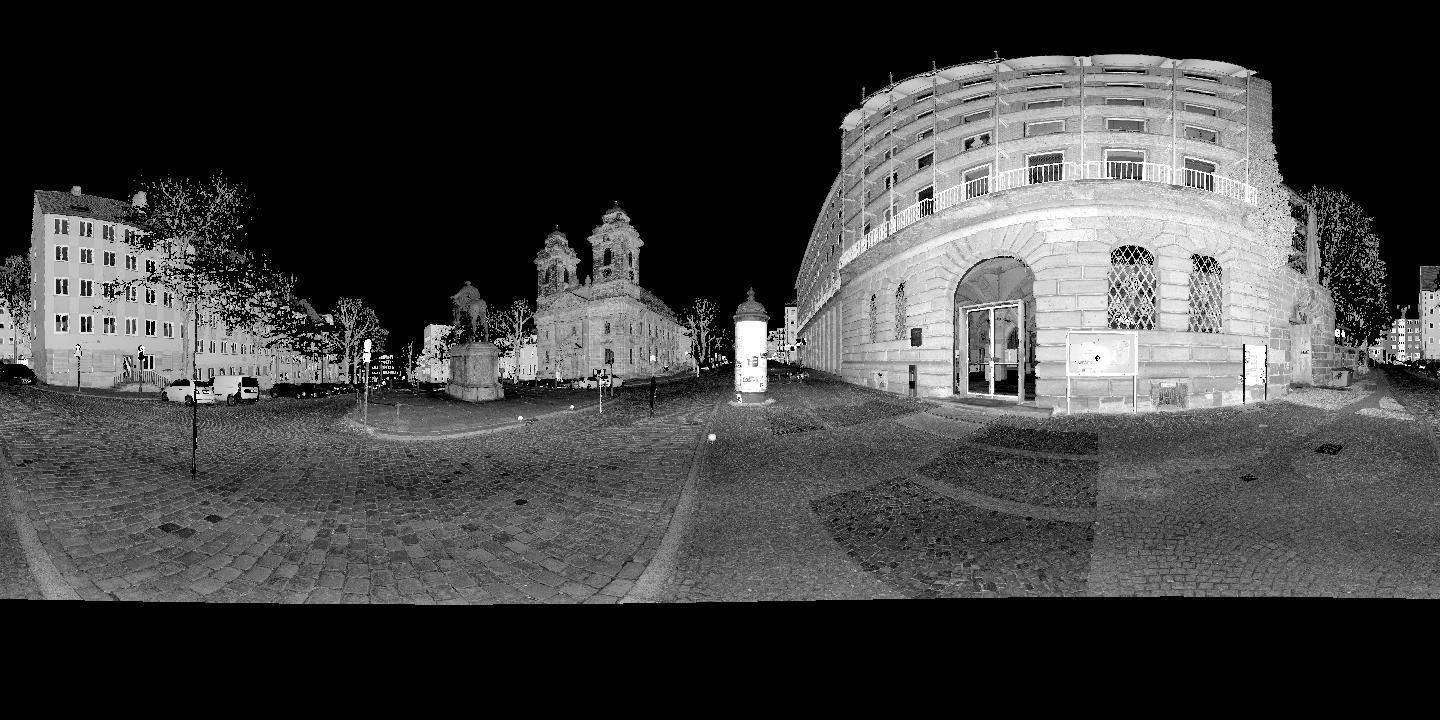
\includegraphics[width=\textwidth]{projection_type_equirectangular.jpg}
		\caption{Equirectangular}
		\label{fig:equirectangular}
	\end{subfigure}
	\hfill
	\begin{subfigure}[b]{0.3\textwidth}
		\centering
		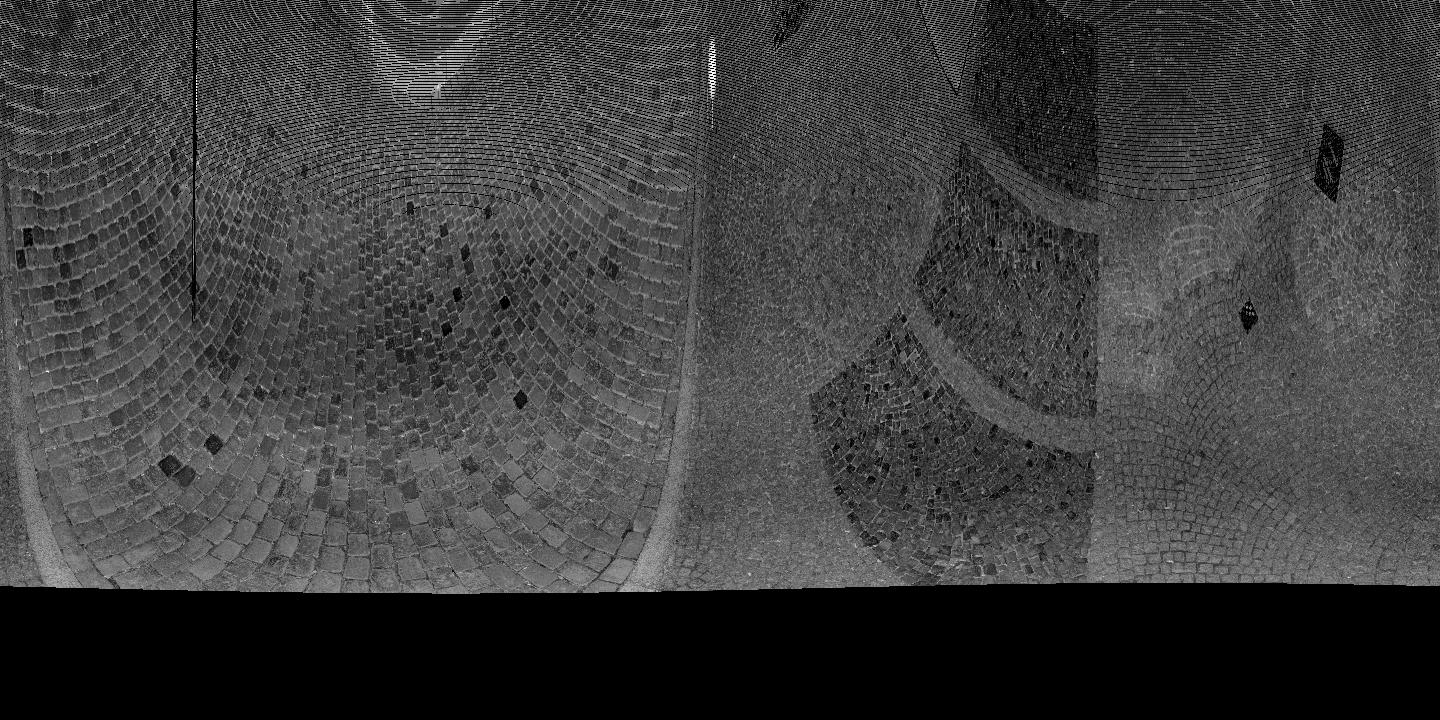
\includegraphics[width=\textwidth]{projection_type_cylindrical.jpg}
		\caption{Cylindrical}
		\label{fig:cylindrical}
	\end{subfigure}
	\hfill
	\begin{subfigure}[b]{0.3\textwidth}
		\centering
		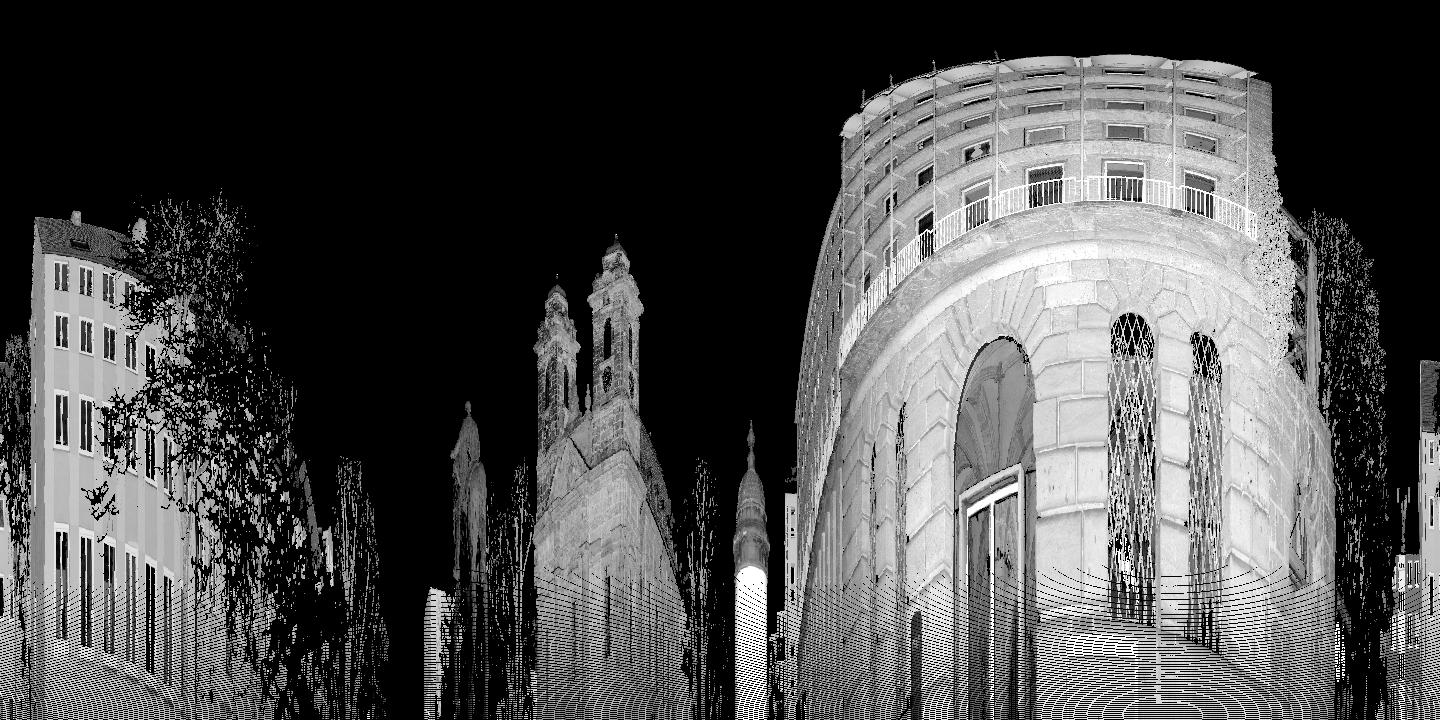
\includegraphics[width=\textwidth]{projection_type_mercator.jpg}
		\caption{Mercator}
		\label{fig:mercator}
	\end{subfigure}
	\caption{Three sample projection types used in PC2B}
	\label{fig:three_projections}
\end{figure}

We have observed that the equirectangular projection is suited best for our purpose (see Figure \ref{fig:equirectangular}). It is one of the most widely spread types and provides full coverage of the scene. Furthermore, it does not apply any transformation or scaling. During testing it proved to be the only useful projection, since the other projections caused many points to stretch into negative infinity. For this reason we used primarily equirectangular projection in this project.
